\lab{Algorithms}{Broyden's Method}{Broyden's Method}

\objective{Implement Broyden's Method and understand the tradeoff with Newton's Method}

We have already discussed using Newton's method to find the roots of an
equation. Newton's method is generally very useful because of its fast
convergence properties. However, Newton's method requires the explicit
calculation of the derivative (i.e., the Jacobian matrix) at each step,
which is computationally costly. There is a class of methods known as quasi-
Newton methods that modify Newton's method so that the derivative (Jacobian)
does not have to be computed at each step, thus making computations faster.
This generally comes at the cost of slower convergence speed, but the increased
computation speed can make these methods more effective in many cases.

One quasi-Newton method is known as Broyden's method. We will first discuss the
one-dimensional case of Broyden's method: the secant method.

The secant method begins with two initial points that are presumably close to
the desired root. We can calculate the equation of the secant line between the
two points $x_i$ and $x_{i-1}$ by the following: \[ y = \frac{f(x_i)-f(x_{i-1
})}{x_i-x_{i-1}}(x-x_i) + f(x_i) \]

Now suppose that we set the next guess of our iterative method to the zero of
the secant line, namely: \[ x_{i+1} = x_i - f(x_i)\frac{x_i-
x_{i-1}}{f(x_i)-f(x_{i-1})} \]

This process is demonstrated in graphically in Figure \ref{Fig:Secant}.  By
continuing this process we (in many cases) will converge to the zero of the
function. This method does not require knowledge of the derivative and hence is
computationally less costly than Newton's method.

This method is shown in pseudocode in Algorithm \ref{Alg:Secant}.

\begin{pseudo}{Secant}{func, x0, x1, tol}
\label{Alg:Secant}
\IF \abs{func(x0)} < tol \THEN
    \RETURN{x0}\\
\IF \abs{func(x1)} < tol \THEN
    \RETURN{x1}\\

\REPEAT 
xnew \GETS x0-func(x0)*\frac{x0-x1}{func(x0)-func(x1)}\\
x0 \GETS x1 \\
x1 \GETS xnew \\
\UNTIL \abs{func(xnew)} < tol \THEN \RETURN{xnew}
\end{pseudo}


\begin{figure}
\begin{center}
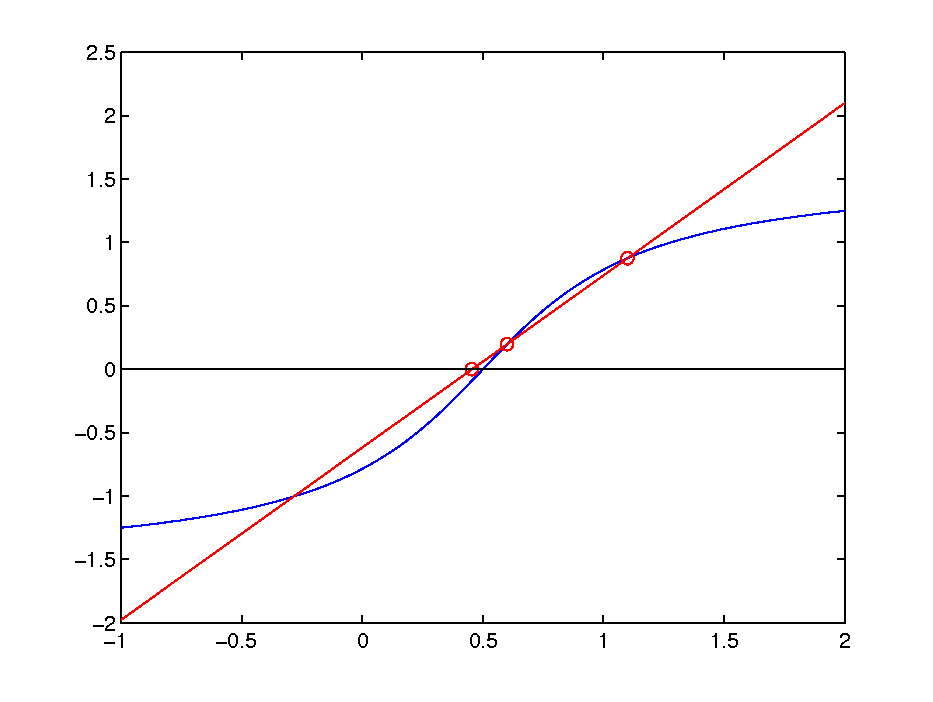
\includegraphics[scale = .5]{Broyden_Secant_Method}
\caption{A demonstration of using the secant method to find a point closer to the desired root.}
\label{Fig:Secant}
\end{center}
\end{figure}	

\begin{problem}
Write a function that takes as input two initial points and a callable function (a function handle or lambda function) and return the zero of the function between the two given points.  If unable to calculate the zero of the function, raise an error.  Also, estimate the exponent of convergence using a log-scaled plot when you use your function to estimate the zero of $e^x-2$. The actual value of the exponent of convergence is a value known as the golden ratio, which can be written:
\[
\phi = \frac{1 + \sqrt{5}}{2} \approx 1.62
\]
The golden ratio shows up in a variety of settings, but we won't discuss them here.
\end{problem}

It is interesting to look at the secant method as a specific case of Newton's method, where we have chosen to approximate the derivative using the secant line between our current set of points.

By combining the secant and the bisection method we obtain a more robust method that is guaranteed to converge. This method is known as the \emph{regula falsi} method. The regula falsi method is thousands of years old, dating to at least the third century BC.

The regula falsi method assumes that we have initial points $x_0$ and $x_1$ such that $f(x_0) < 0 < f(x_1)$. We then use the root of the secant line to find our new point $x_2$. However, we then choose to keep $x_1$ only if $\mbox{sgn}(f(x_2)) \neq \mbox{sgn}(f(x_1))$, otherwise we keep $x_0$. In this manner we can combine the robustness of the bisection method with some of the faster convergence properties of the secant method.

\begin{problem}
Write a function implementing the regula falsi method. Compare convergence speed with the secant method on the functions:
\begin{align*}
f(x) &= e^x-1\\
f(x) &= cos(x)\\
f(x) &= x^7\\
\end{align*}
\end{problem}

%-----------------------Need Clarification (Jacobian)-----------------------
The generalization of the secant method to multiple dimensions is called Broyden's Method.  If we have the point $x_k$ and the Jacobian $J_k$ at that point we can use the following equation to select our guess for the zero of the function:
\begin{equation} \label{Eq:BroydenSolve}
J_k \Delta x = -F(x_k)
\end{equation}

Where $\Delta x = x_{k+1}-x_k$. This is precisely Newton's method. However, since calculating the Jacobian at each step is costly, we instead use a generalization of secant lines to estimate the Jacobian (just as we used a secant line to approximate the derivative in the one-dimensional case).

The generalization for using secant lines is as follows: If we have points $x_k$ and $x_{k-1}$ then the Jacobian $J_k$ at the point $x_k$ will approximately satisfy the following equation:
\begin{equation}
J_k (x_k-x_{k-1}) \approx F(x_k) - F(x_{k-1})
\end{equation}
In the one dimensional problem we can use this equation to exactly specify the value $J_k$ (this is simply a finite difference approximation of the derivative). However, in multiple dimensions, the equation will be underdetermined (i.e. many $J_k$'s will satisfy the equation). However, suppose that we have a previous estimate of the Jacobian $J_{k-1}$ at the point $J_{k-1}$. We can then find the solution to the multi-dimensional secant equation above that minimizes $\|J_{k-1}-J_k\|$. This requirement is uniquely fulfilled by the following:
\begin{equation} \label{Eq:BroydenJacobian}
J_k = J_{k-1} + \frac{\Delta F-J_{k-1} \Delta x}{\|\Delta x\|^2}\Delta x^T
\end{equation}

In this equation the $\Delta F = F(x_k)-F(x_{k-1})$ and $\Delta x = x_k-x_{k-1}$. Intuitively, we are using the secant equation to make a rank-one update on the Jacobian at each step of the algorithm.

After we have obtained our secant line approximation of the Jacobian (Equation \ref{Eq:BroydenJacobian}) we can apply Equation \ref{Eq:BroydenSolve} to find $x_{k+1}$. We can then repeat this process until we have (presumably) converged to a zero of the function. Pseudocode is shown in Algorithm \ref{Alg:Broyden}:

\begin{pseudo}{Broyden}{func,x1,x2,tol}
\label{Alg:Broyden}
\IF \abs{func(x1)} < tol \THEN
    \RETURN{x1}\\
\IF \abs{func(x2)} < tol \THEN
    \RETURN{x2}\\

J \GETS Jacobian(x1) \\

\REPEAT 
F1 \GETS func(x1) \\
F2 \GETS func(x2) \\
\Delta x \GETS x2 - x1 \\
J \GETS J + \frac{F2-F1-J \Delta x}{\|\Delta x \|^2}\Delta x^T \\
xnew \GETS J^{-1} (-F2) + x2 \\
x1 \GETS x2 \\
x2 \GETS xnew \\
\UNTIL \abs{func(xnew)} < tol \THEN \RETURN{xnew}
\end{pseudo}

\begin{problem}
Write code implementing Broyden's method. Test it on the function:
\[
f(x,y,z) = 
 \left( \begin{array}{ccc}
cos(xy)+ xz^3 \\
y^2 - y + x^2 \\
z + x-\frac{1}{2}-\sqrt[3]{2cos(\frac{1}{4})} \end{array} \right)
\]
using starting points $(1,2,3)$ and $(3,2,1)$
\end{problem}

We can often make Broyden's method faster using the Sherman-Morrison Woodbury Formula. This formula allows us to efficiently calculate the inverse of a matrix when we add a low rank update to that matrix. After manipulation of the Sherman-Morrison Woodbury Formula we obtain the following:

\[
J_k^{-1} = J_{k-1}^{-1} + \frac{\Delta x_k - J_{k-1}^{-1}\Delta F_k}{\Delta x_k^T J_{k-1}^{-1}\Delta F_k} (\Delta x_k^T J_{k-1}^{-1})
\]

Thus, we can calculate the inverse of the Jacobian in the first step of our algorithm and then calculate an update to the inverse at each step using the above formula.

\begin{problem}
Implement this modification in a new file. Now compare the two versions of Broyden's method on the function above. Which is faster? Are there cases where one implementation is better than the other?
\end{problem}
